%! TEX root = ../aminhash.tex

\section{Experiments}\label{sec:evaluation}

In this section, we show that our proposed estimators lead to improved performance on maximum
Jaccard similarity search on real datasets.
All code is available at~\cite{codes}, implemented in Python with critical parts written in Cython for near C level speed.

We run our experiments on the Flickr, DBLP and Netflix dataset from a recent set-similarity join survey by Mann et al.~\cite{mann2016empirical}.
These datasets were also used by \cite{christiani2018scalable} and \cite{ahle2020problem}.
In the survey these datasets were identified as archetypical examples with and without Zipf-like behaviour.
Mann et al. write:
 ``Most datasets, like FLICKR (cf. Figure 7), show a Zipf-like
 distribution and contain a large number of infrequent tokens (less
 than 10 occurrences), which favors the prefix filter. In contrast,
 NETFLIX has almost no tokens that occur less than 100 times,''
In practice, this means that the Netflix dataset requires a much larger $K$, for reasonable recall than the Flickr dataset, but we still get substantial improvements in recall on both.
%The Netflix dataset is originally from \href{https://www.cs.uic.edu/~liub/Netflix-KDD-Cup-2007.html}{KDD-Cup 2007}.

\subsection{Recall vs Memory usage}





% First, we fix the quantization
% mechanism and compare traditional reconstruction
% loss with our proposed loss to show that score-aware
% loss leads to better retrieval performance and more accurate estimation of maximum inner product values.
% Next, we compare in fixed-bit-rate settings against
% QUIPS and LSQ, which are the current state-of-the art for many MIPS tasks. Finally, we analyze the
% end-to-end MIPS retrieval performance of our algorithm in terms of its speed-recall trade-off in a
% standardized hardware environment. We used the
% benchmark setup from ann-benchmarks.com, which
% provides 11 competitive baselines with pre-tuned parameters. We plot each algorithm's speed-recall curve
% 
% 

We are interested in how the number of hash values per stored set trades with the recall.
The number of such values is directly proportional to the memory required to store the dataset.
%We measure memory in the number of independent hash functions we need to store values from.
%\footnote{Each value can be stored in a word, and it is possible to compress them further, usually down to around a byte without loss of accuracy.}
We focus on the measure recall@10, which means how often the estimated top 10 most similar sets contain the true most similar set.
If the searcher wants to obtain the true nearest set, they can use the estimation as a fast first scan over the data, and then compute the true similarities between the query and the 10 candidates.
For optimal speed the engineer wants to trade-off $K$ for the number of candidates that need to be ``rescored'', so recall@30 or 100 may also be interesting.
We picked 10 for our experiments because of its standard use in benchmarks~\cite{aumuller2017ann}.

For each experiment, we shuffled the dataset and split it into 10,000 sets for queries and the remaining for the database.
The database was hashed using $K$ independent MinHash functions.
The shuffling and hash functions use the same randomness across experiments with different datasets.
% Experimentally we find that we can increase recall@10 by 50\% at small values of $K$.
%The following shows the effect on recall@10 with 10,000 queries:
We picked a handful of typical $K$ values and estimated the distances with the classical estimator, the maximum likelihood estimator, and the Minner estimator with respectively 0, 1 and 8 iterations of Newton's method.
For Flickr we picked lower $K$ values since the recall got very high very quickly.
The results are shown in tables \ref{tab:netflix}, \ref{tab:flickr} and \ref{tab:dblp}.

In every experiment, the Minner estimator beat the classical estimator, and for larger $K$ the MLE or Minner estimator with Newton iterations was best.
Using 8 iterations of Newton's method was usually slightly better than running 1, but the difference was minor compared to 0 vs 1 iteration.

\smallskip

The results are a bit hard to interpret, since a $98\%$ to $99\%$ improvement may be much harder to get than a $40\%$ to $44\%$, even if the later is 4 times bigger in terms of percentage points gained.
Instead, we opt to measure improvement in terms of how many more MinHash values we would have needed with the classical estimator to obtain the recall of our best estimator.
This has the advantage of corresponding directly to space saved.

To measure the improvement in terms of increased $K$ values,
we assume a simple non-negative logistic model $\text{recall@10} = 1 - \exp(-K/a)$ for some constant $a$ depending on the estimator and the dataset.
Thus for recall $r$ we need $K=a\log\frac1{1-r}$ MinHash Values.
For a given recall $r$ the improvement of model $a_1$ over $a_2$ in terms of $K$ is thus a factor $a_1/a_2$.

We perform regressions (with least squares) based on this model and the data in tables \ref{tab:netflix}, \ref{tab:flickr} and \ref{tab:dblp}.
For Netflix, we get $a_\text{classic}=300.7$ and $a_\text{best} = 233.9$ showing an improvement of $28.5\%$ in terms of $K$ values.
For Flickr, we get $a_\text{classic}=10.73$ and $a_\text{best} = 9.644$, corresponding to an $11.3\%$ improvement,
and for DBLP, we get $a_\text{classic}=204.2$ and $a_\text{best}=168.3$, a $21.4\%$ improvement.

Alternative we could have used a normal logistic model $r = 1/(1 + \exp(-K/a))$.
Fitting our data with this model results in larger improvements of resp. $53.1\%$, $27.5\%$ and $14.5\%$.
However the model is a bad fit, since it has $r\ge 1/2$ for all $K\ge 0$.
We could fix this by adding a constant term and use $r=1/(1+\exp(b-K/a))$, however then the ratio of improvement is no longer independent of $r$.

% Data with positive logistic model:
% (py38) thdy@preciousss:~/asymmetric-minhash/code$ py regression.py flickr
% [10.73395277]
% [9.64429099]
% [0.11298516]
% [0.10151542]
% (py38) thdy@preciousss:~/asymmetric-minhash/code$ py regression.py netflix
% [300.68230093]
% [233.91258753]
% [0.28544729]
% [0.22206067]
% (py38) thdy@preciousss:~/asymmetric-minhash/code$ py regression.py dblp
% [204.22362543]
% [168.26528607]
% [0.21370028]
% [0.17607336]

% Normal logistic model
% Dblp
%[229.83233232]
%[180.38555126]
%[0.27411719]
%[0.21514284]
% Netflix
%[428.99438321]
%[280.23065982]
%[0.5308617]
%[0.34677313]
% Flickr
%[11.79897987]
%[10.30467806]
%[0.14501198]
%[0.1266467]


%Some timing data:
%Tid for -K 100 --newton 1
%Time preparing: t1=2813.205824613571, Time searching: t2=5754.812134742737
%Tid for -K 100 --newton 2
%Time preparing: t1=2768.65847158432, Time searching: t2=5648.562669038773
%Tid for -K 100 --newton 4
%Time preparing: t1=2715.9863698482513, Time searching: t2=5616.8901562690735
%Tid for -K 100 --newton 8
%Time preparing: t1=2769.066630601883, Time searching: t2=6230.902306318283
%
%-K 1 --newton 8
%Time preparing: t1=31.681596994400024, Time searching: t2=765.3667838573456

\begin{table}
\centering
 \begin{tabular}{|r| r r r r r|} 
 \hline
     \multicolumn{6}{|c|}{Recall@10 on the Netflix dataset} \\
 \hline
 K  & Classic & MLE & Minner & Minner 1N & Minner 8N \\
 \hline
    1 & 0.0033 & 0.0076 & \textbf{ 0.0099} & 0.0057 & 0.0063 \\
  10 & 0.0501 & 0.0396 & \textbf{ 0.0623} & 0.0506 & 0.0462 \\
  30 & 0.1474 & 0.1773 & \textbf{ 0.1914} & 0.1910 & 0.1862 \\
  100 & 0.3831 & 0.48($\ast$)
  & 0.4640 & 0.4870 & \textbf{ 0.4903} \\
  400 & 0.7510 & 0.83($\ast$) & 0.8054 & 0.8326 & \textbf{ 0.8338} \\
  500 & 0.7942 & 0.85($\ast$) & 0.8440 & 0.8660 & \textbf{ 0.8667} \\
  \hline
 \end{tabular}
 \caption{The Minner estimator is best at small $K$, but eventually the asymptotics kick in and the Maximum likelihood estimator overtakes. The MLE is very slow however, and one can get most of the benefits by applying a single iteration of Newton's method on top of the Minner estimator.
    For the midrange $K$ values 30 and 100 we get a near 30\% improvement in recall over the classical estimator.
   ($\ast$): MLE results for large $K$ were stopped after 2000 queries and 48 hours.
 }
 \label{tab:netflix}
\end{table}

\begin{table}
\centering
 \begin{tabular}{|r| r r r r r|} 
 \hline
     \multicolumn{6}{|c|}{Recall@10 on the Flickr dataset} \\
 \hline
 K  & Classic & MLE & Minner & Minner 1N & Minner 8N \\
 \hline
    1 & 0.2379 & 0.3410 & \textbf{ 0.3595} & 0.2806 & 0.2969 \\
   5 & 0.6256 & 0.5457 & \textbf{ 0.6688} & 0.5913 & 0.6138 \\
  10 & 0.7770 & 0.7155 & \textbf{ 0.8122} & 0.7327 & 0.7469 \\
  20 & 0.8657 & 0.8540 & \textbf{ 0.8963} & 0.8217 & 0.8352 \\
  30 & 0.9108 & 0.9080 & \textbf{ 0.9301} & 0.8597 & 0.8714 \\
  \hline
 \end{tabular}
 \caption{The Flickr dataset is much easier than the Netflix dataset and as such doesn't require as many MinHash values to obtain a good recall. The Maximum likelihood estimator never overcomes its asymptotic disadvantage, but the Minner estimator improves 2-7\% in recall over the classic estimator, and all of $51\%$ at $K=1$.}
 \label{tab:flickr}
\end{table}


\begin{table}
\centering
 \begin{tabular}{|r| r r r r r|} 
 \hline
     \multicolumn{6}{|c|}{Recall@10 on the DBLP dataset} \\
 \hline
 K  & Classic & MLE & Minner & Minner 1N & Minner 8N \\
 \hline
    1 & 0.0036 & 0.0097 & \textbf{ 0.0105} & 0.0071 & 0.0080 \\
  10 & 0.0987 & 0.0998 & 0.1057 & 0.0993 & \textbf{ 0.1072} \\
  30 & 0.2978 & 0.3438 & 0.3264 & 0.3445 & \textbf{ 0.3524} \\
 100 & 0.5736 & 0.6460 & 0.6145 & 0.6519 & \textbf{ 0.6536} \\
 400 & 0.8676 & 0.90($\ast$) & 0.8932 & 0.9148 & \textbf{ 0.9153} \\
 500 & 0.9009 & 0.93($\ast$) & 0.9214 & 0.9380 & \textbf{ 0.9385} \\
  \hline
 \end{tabular}
 \caption{The DBLP dataset appears somewhere in between Netflix and Flickr in terms of difficulty.
    On DBLP the MLE (or Minner with Newton iterations) generally does better than pure Minner.
   ($\ast$): MLE results for large $K$ were stopped after 2000 queries and 48 hours.
 }
 \label{tab:dblp}
\end{table}

%\subsection{Estimation: Hash functions vs Accuracy}
\subsection{Estimation}\label{sec:estimation}

\begin{figure}
   \centering
   % trim is left bottom right top
   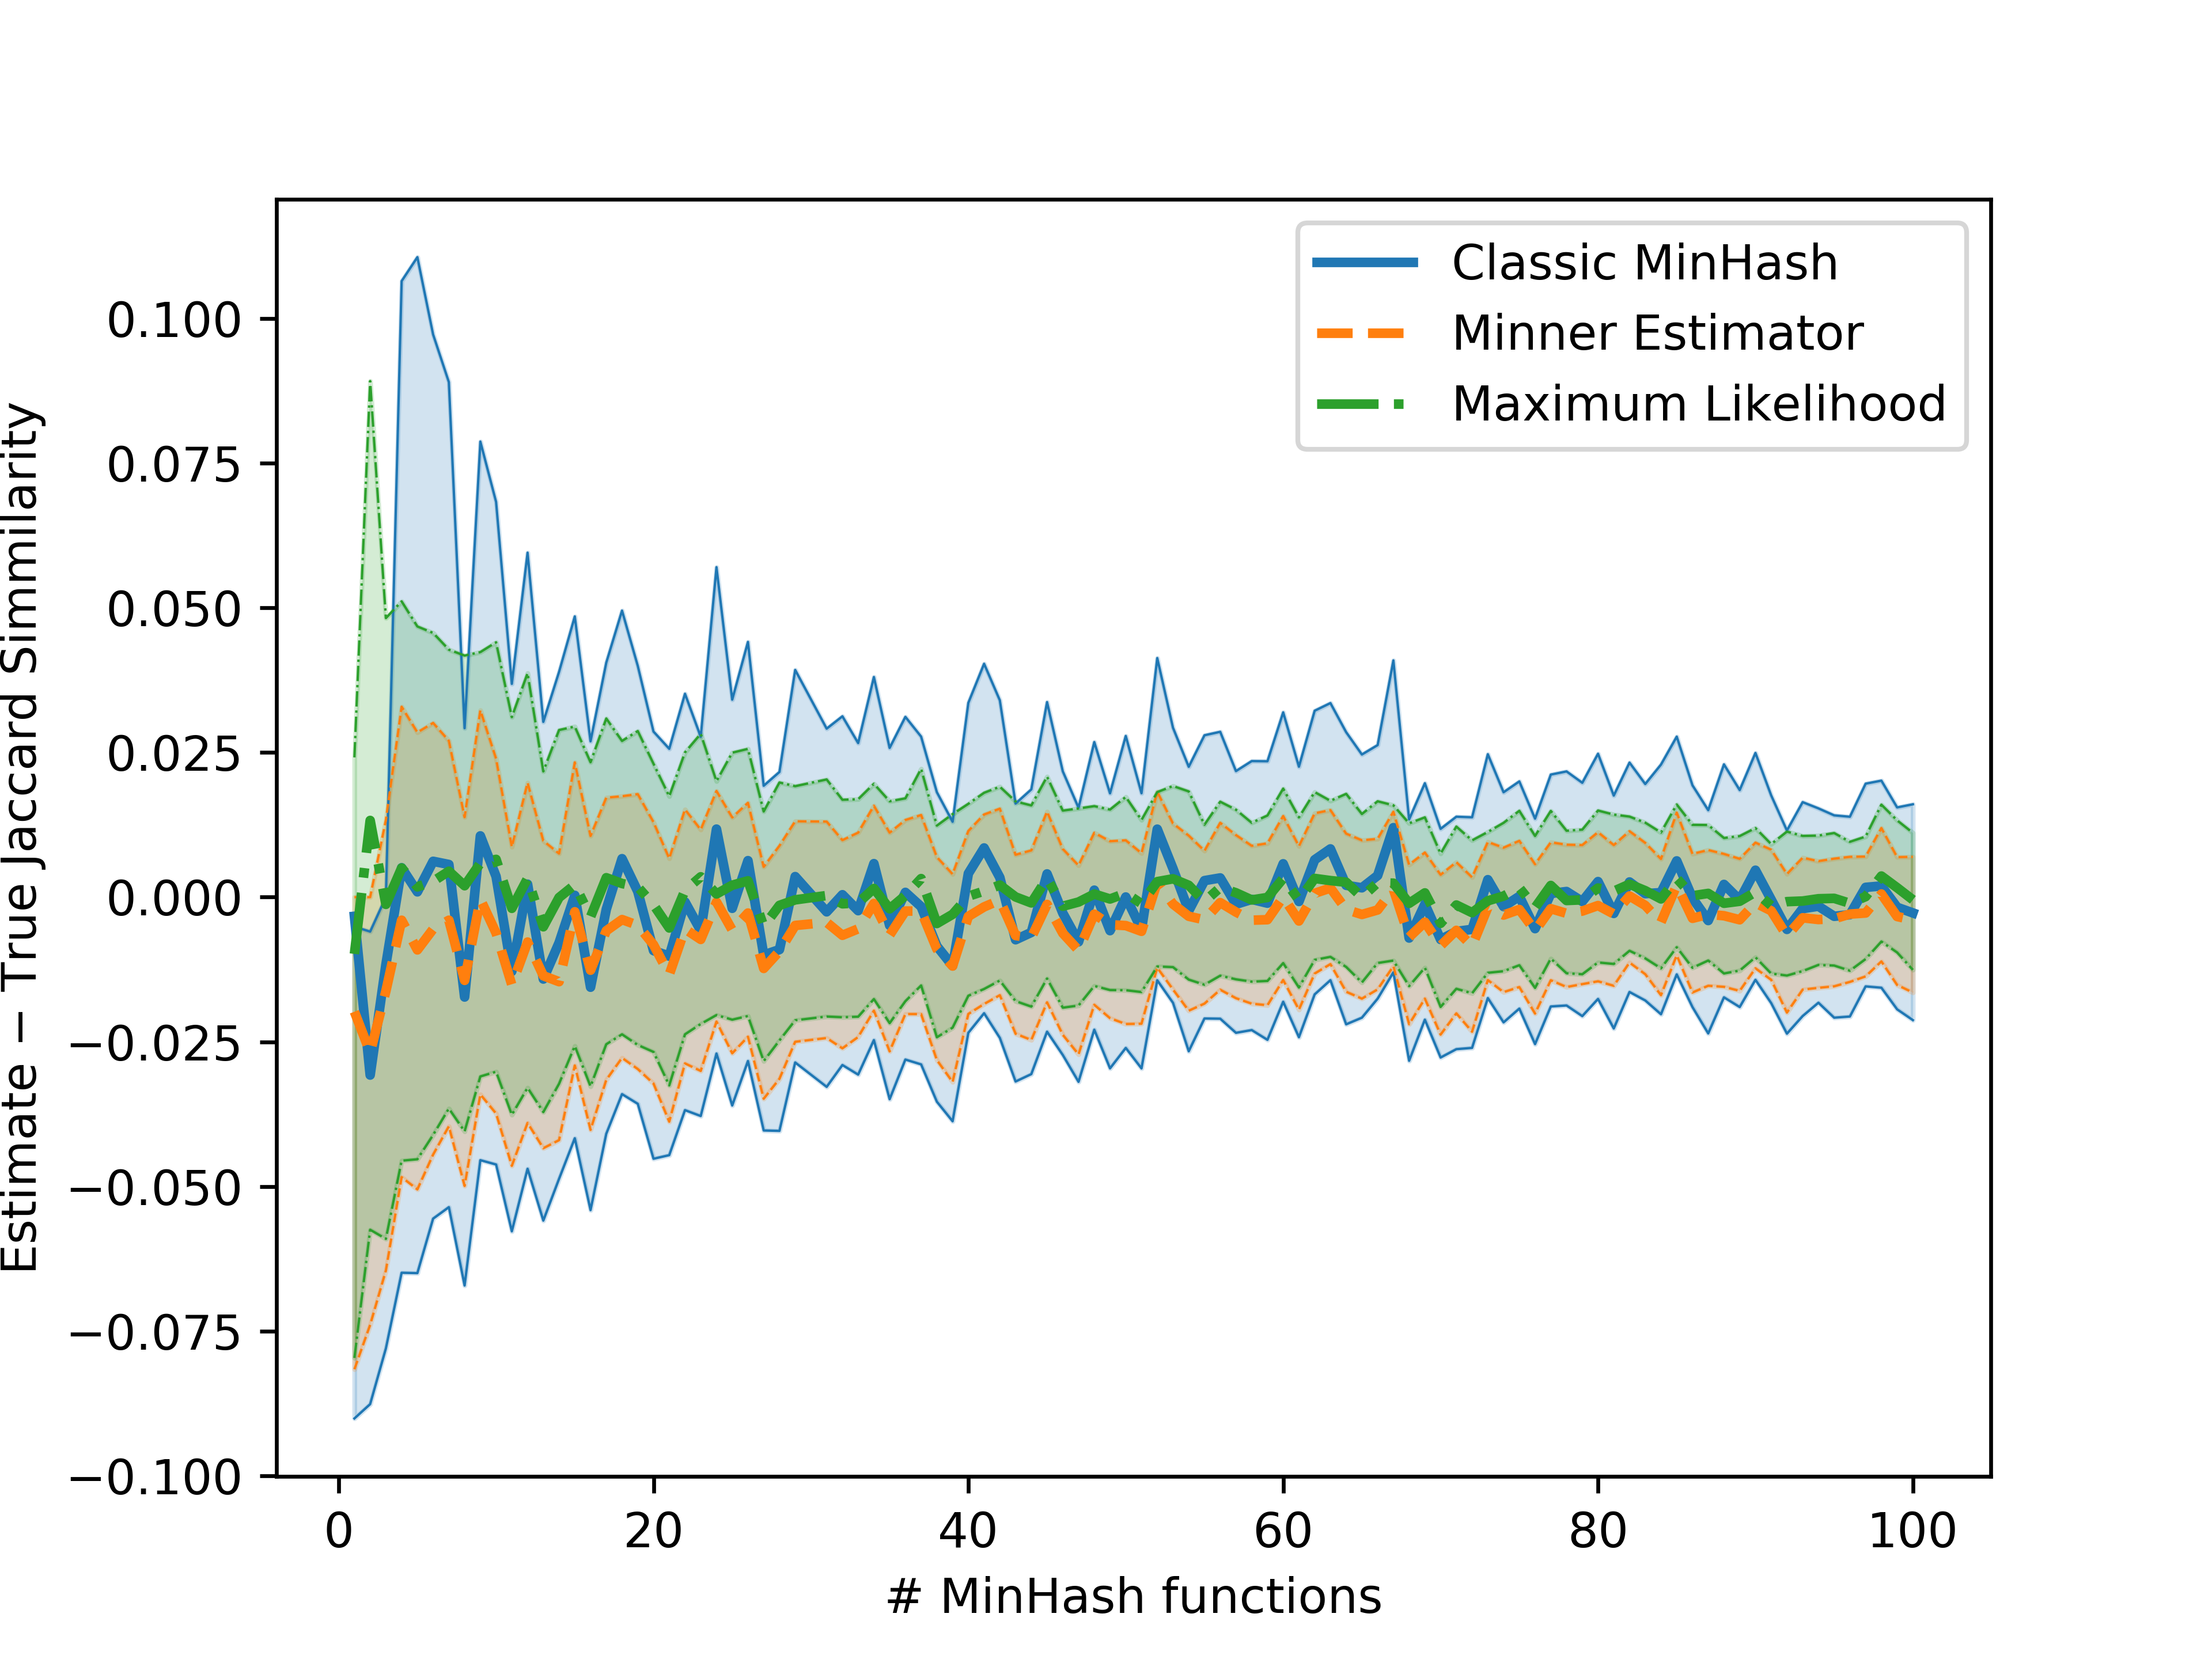
\includegraphics[trim=0 0 35 40,clip,width=\linewidth]{figures/var2}
   \caption{
      Mean values with 1 standard deviation bounds (15.9\% percentile)
      on the estimation error for 5 million pairs from the Netflix dataset.
   }
   \label{fig:var}
\end{figure}

The other natural experiment to perform is measuring the difference between estimated similarity and real similarity.
\Cref{fig:var} is inspired by~\cite{thorup2013bottom}.
We sampled 50 random queries from the dataset and estimated the similarity to all other sets.
For each batch, we subtracted the real similarity and computed mean and percentiles.
While this is not the main focus of the paper, we note that the results are consistent with the variance computed for the MLE and our experimental variance computations in~\cref{fig:exp_variance}.

The code for every plot is available at~\cite{codes} as well.
